\documentclass{report}[a4paper,12pt] %article,book,report

% Package Imports
\usepackage{amsmath} % Equations
\usepackage{graphicx} % Image Management
\usepackage{subcaption}
\usepackage{lipsum} % Random Text
\usepackage{hyperref} % Hyper Links
\usepackage{booktabs} % For prettier tables
\usepackage{minted} % Code Formatting
\usepackage{enumitem} % Customize List Bullets

% Config
\graphicspath{{../../../../../common/images/stock/}}

\hypersetup{
    colorlinks=true,
    linkcolor=blue,
    filecolor=magenta,      
    urlcolor=red,
    pdftitle={Latex Tutorial},
    pdfpagemode=FullScreen,
    }

% Preamble: Title Details
\title{Latex Tutorial}
\date{2023-10-25}
\author{Amanpreet Singh}

\begin{document}
  \pagenumbering{arabic}
  \maketitle %Insert Title
  \tableofcontents
  \newpage %Break Page

%\part{One}
\chapter{Basics} %book,report only
\section{Introduction}
This is the introduction section.
\href{http://www.latex-tutorial.com}{LaTeX-Tutorial} is being followed.
\href{https://www.overleaf.com/learn}{Overleaf} also has good guide.

\paragraph*{Latex} allows you to typeset document quickly using smart markup language.
There are many plugins (packages) available to enhance functionality.

\subsection{Subsection}
This is a subsection.  
Organisation of Content is done in this manner, \href{https://www.overleaf.com/learn/latex/Sections_and_chapters}{guide}.

\subsubsection{Sub Subsection}
This is a sub-subsection.

\paragraph{Paragraph} 
This is a Paragraph.

\subparagraph{Sub Para}
This is a Sub Paragraph

\section{Features}

\subsection{Math}

\paragraph{Equations}
Equations Package Example.
\begin{equation}
  f(x) = x^2
\end{equation}

\paragraph{Embedding}

This formula $f(x) = x^2$ is an embedding.

\paragraph*{Double Line}

\begin{equation*}
  1 + 2 = 3 
\end{equation*}

\begin{equation*}
  1 = 3 - 2
\end{equation*}

\begin{align*}
  1 + 2 &= 3\\
  1 &= 3 - 2
\end{align*}

\paragraph{Fractions}

\begin{align*}
  f(x) &= x^2\\
  g(x) &= \frac{1}{x}\\
  F(x) &= \int^a_b \frac{1}{3}x^3
\end{align*}

Refering to Foot Note\footnote{\label{myfootnote}Tutorial footnote}.

\subsection{Formatting}

Various \hypertarget{sen:formatopts}{Formattings} are Available.
\paragraph{Basic} Formatting Options using Tags.
\begin{enumerate}
  \item \textbf{Bold}
  \item \textit{Italics}
  \item \underline{Underline}
  \item \emph{Emphatic}
  \item `Single Quote'
  \item ``Double Quote''
  \item Special Chars, \verb|*`-$&|
\end{enumerate}

\paragraph{Alignment} Can be done using align block. 
\verb|*| Indicates not to put number for that Section.

\begin{align*}
  \text{Left Align}\\
  \text{Right aligned}
\end{align*}

I'm referring to footnote again using \verb|\ref| \ref{myfootnote}.

\subsection{References}
There are many ways to reference. We use package `hyperref'.
\begin{enumerate}
  \item Direct URL \url{https://www.overleaf.com/learn/latex/Hyperlinks}
  \item Hyper Link: \href{https://www.overleaf.com/learn/latex/Hyperlinks}{Hyperlink Guide}
  \item Link to Sentence
  \item File Link: \href{run:../../presentation/beamer/tutorial.tex}{Beamer Example}
  \item Reference to a label \ref{lst:bullet}.
  \item Page Reference: \pageref{fig:coffee}
  \item Word or \hyperlink{sen:formatopts}{sentence} in your document.
\end{enumerate}

\newpage
\subsection{Images}

\paragraph{Placement Specifiers} control \href{https://www.overleaf.com/learn/latex/Positioning_images_and_tables#The_figure_environment}{placement} of image and tables.
\verb|h!| indicates to place image where it appears. Try `New Page' if it is not being honored.

Images can also be in multiple folders. \verb|\graphicspath{ {./images1/}{./images2/} }|.
Size, rotation can be \href{https://www.overleaf.com/learn/latex/Inserting_Images}{tuned} as well.

\paragraph{Single}

Figure \ref{fig:sailboat} shows a boat. %Refers Label

\begin{figure}[h]
  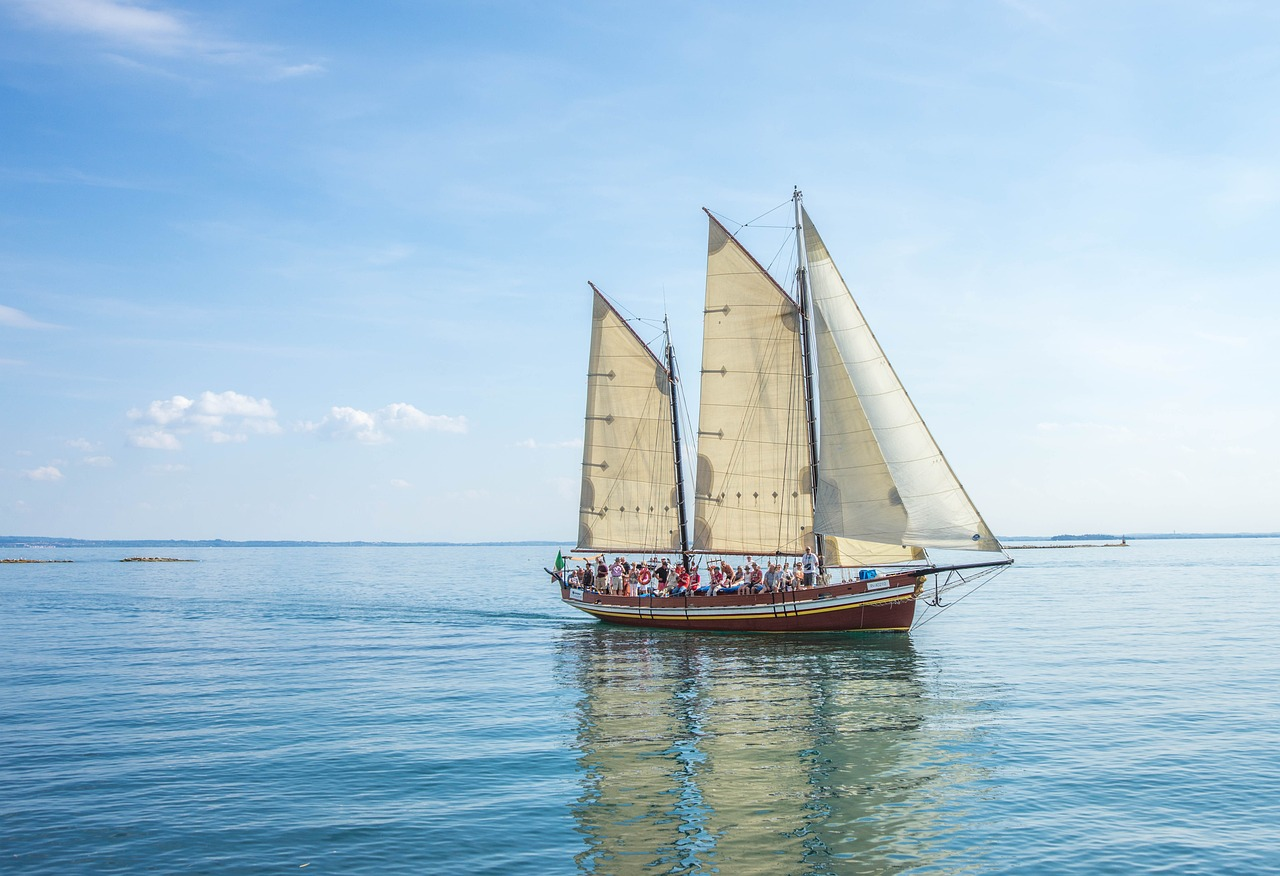
\includegraphics[width=\linewidth,scale=1.5]{boat.jpg}
  \caption{Sail Boat.}
  \label{fig:sailboat} %Invisible Used for Reference
\end{figure}

\newpage
\paragraph{Multiple}
Figure \ref{fig:coffee} shows how to place image side by side.

\subparagraph{Images aligned} next to each other, their widths are both set to \textbf{0.4}, yet they fill up the whole space.
You should always set this value to .1 less than you expect.

\begin{figure}[h!]
  \centering
  \begin{subfigure}[b]{0.4\linewidth}
    
\includegraphics[width=\linewidth]{coffee.jpg}
    \caption{Coffee.}
  \end{subfigure}
  \begin{subfigure}[b]{0.4\linewidth}
    
\includegraphics[width=\linewidth]{coffee.jpg}
    \caption{More coffee.}
  \end{subfigure}
  \caption{Two Coffies}
  \label{fig:coffee}
\end{figure}

If you want to align three images next to each other,
you should consecutively add three subfigures, each with a \verb|.2\linewidth|


\paragraph{Cluster}
Figure \ref{fig:coffee3} shows how to place cluster of images.

\subparagraph{Notice} images are Numbered Automatically.

\begin{figure}[h!]
  \centering
  \begin{subfigure}[b]{0.2\linewidth}
    
\includegraphics[width=\linewidth]{coffee.jpg}
     \caption{Coffee.}
  \end{subfigure}
  \begin{subfigure}[b]{0.2\linewidth}
    
\includegraphics[width=\linewidth]{coffee.jpg}
    \caption{Tasty coffee.}
  \end{subfigure}
  \begin{subfigure}[b]{0.2\linewidth}
    
\includegraphics[width=\linewidth]{coffee.jpg}
    \caption{More coffee.}
  \end{subfigure}
  \begin{subfigure}[b]{0.5\linewidth}
    
\includegraphics[width=\linewidth]{coffee.jpg}
    \caption{Too much coffee.}
  \end{subfigure}
  \caption{Coffee Cluster}
  \label{fig:coffee3}
\end{figure}

\subsection{Tables}

\paragraph{Useful} Resources
\begin{align*}
  \href{https://tableconvert.com/latex-generator}{Table Generator}\\
  \href{https://www.tablesgenerator.com/latex_tables}{Book Table Generator}\\
  \href{https://latex-tutorial.com/tutorials/tables/}{Tutorial}
\end{align*}

\paragraph*{Packages} for Tables
\begin{enumerate}
  \item Prettify your tables using the booktabs package.
  \item Make your tables span multiple pages with the longtable package
  \item Display your tables in landscape using the rotating package  
\end{enumerate}

\begin{table}[!h]
  \centering
  \caption{Basic Table}
  \begin{tabular}{|l|l|}
  \hline
      \textbf{Heading 1} & \textbf{Heading 2} \\ \hline
      Hello & World \\ \hline
  \end{tabular}
  \label{tab:basic}
\end{table}

\begin{table}[h!]
  \begin{center}
    \caption{Alighned Table}
    \label{tab:alighned}
    \begin{tabular}{l|c|r} % <-- Alignments: 1st column left, 2nd middle and 3rd right, with vertical lines in between
      \textbf{Value 1} & \textbf{Value 2} & \textbf{Value 3}\\
      $\alpha$ & $\beta$ & $\gamma$ \\
      \hline
      1 & 1110.1 & a\\
      2 & 10.1 & b\\
      3 & 23.113231 & c\\
    \end{tabular}
  \end{center}
\end{table}

\begin{table}[h!]
  \centering
  \caption{Book Table}
  \label{tab:book}
  \begin{tabular}{@{}lcr@{}} %<-- Left, Center, Right
    \toprule % <-- Toprule here
    \textbf{Value 1} & \textbf{Value 2} & \textbf{Value 3}\\
    $\alpha$ & $\beta$ & $\gamma$ \\
    \midrule % <-- Midrule here
    1 & 1110.1 & a\\
    2 & 10.1 & b\\
    3 & 23.113231 & c\\
    \bottomrule % <-- Bottomrule here
  \end{tabular}
\end{table}

\subsection{Lists}
Lists are easy to create:
\paragraph{Bullets}

\begin{itemize}
  \label{lst:bullet}
  \item List entries start with the \verb|\item| command.
  \item Individual entries are indicated with a black dot, a so-called bullet.
  \item The text in the entries may be of any length.
  \item Below is an example of Nested List.
  \begin{itemize}
    \item Sub List 1
    \item \lipsum[1]
    \item Sub List 3
  \end{itemize}
\end{itemize}

\paragraph{Ordered}
This is an example of Ordered Lists.

\begin{enumerate}[label=(\roman*)]
  \label{lst:order}
  \item Latex is much more powerful than Markdown.
  \item It has lot more options as compared to markdown.
  \item Markdown syntax is simple but also limited.
  \begin{description}
    \item[Note:] This allows me to add such sections.
    \item[Tip!] Most of the complex Syntax is handled via IDE.
  \end{description}
\end{enumerate}

\paragraph{Custom} bullet points can be set. Many \href{https://latex-tutorial.com/bullet-styles/}{Styles} are available.
Package `enumitem' helps customize it for Ordered List \ref{lst:order} as well.
\begin{itemize}
  \label{lst:format}
  \item[--] Dash
  \item[$-$] Dash
  \item[$\ast$] Asterisk
\end{itemize}

\chapter{Tools}
\section{Code}
\paragraph{Minted} Packages allows to format and display Code.

\begin{enumerate}
  \item Code Snippet \ref{code:snippet} and File. \ref{code:file}
  \item Code can also be given inline \verb|\mintinline{c}|fmt.Println("Hello")|| (Not Working)
\end{enumerate}

\subsubsection{Snippet}
\begin{listing}[h]
  \begin{minted}{Python}
    def hello_world():
    print("Hello floating World!")
  \end{minted}
  \caption{Code Snippet}
  \label{code:snippet}
\end{listing}

\subsubsection{Beamer Latex}
\label{code:file}
\paragraph{Code} file example for Minted.
\inputminted{tex}{../../presentation/beamer/tutorial.tex} 

\section{Editor}
Tool of choice is \href{https://github.com/James-Yu/LaTeX-Workshop}{Latex Workshop} in Vscode.
\subsection{Hotkeys}
\begin{itemize}
  \item Use Insert Snippet to Access Surround Settings.
  \item SyncTex from Cursor can be used to focus current PDF Location where edit is Happening.
  \item Auto Complete is Triggered both on \verb|\|
  \item Other Auto Completions have Sensible Prefixes. Example
  \begin{itemize}
    \item `B' for Begin Sections
    \item `F' for Font Completions
    \item `S' for Sections and Para's
    \item `M' for Math.
    \item `BT' for Tables
  \end{itemize}
\end{itemize}

\subsection{Settings}
\begin{itemize}
  \item Settings allow you to enable SyncTex (Pdf Focus) on Generate.
  \item Can add Custom Trigger Chars for Autocomplete.
  \item Follow Cursor in Structure Section moves to correct heading is Structure.
  \item Minted requires \verb|--shell-escape| follow Vscode \href{https://leportella.com/minted-vscode/}{Guide}.
\end{itemize}

\subsection{Tips}
\begin{itemize}
  \item Can use Side Bar to Get Structure and easy Navigate.
  \item Collapsing Sections is possible.
  \item \textbf{Word Count} can be used to do word check
  \item Snippet View (Under) Structure helps insert Special/Math Symbols.
  \item \href{https://github.com/James-Yu/LaTeX-Workshop/wiki/Compile#cleaning-generated-files}{Clean} Auxilary file removes Temp Files and Autoclean
  \item Customize `latex-workshop.shortcut' Shourtcuts for easy formatting.
\end{itemize}


\section*{Appendix}
\begin{appendix}
  \listoffigures
  \listoftables
\end{appendix}

\end{document}